\documentclass[12pt,AutoFakeBold]{article} 

% 注意:本模板还是存在一定的问题的,指导老师评语和实验报告内容基本要求之间本不应该有空隙,但我不会处理,但这个小问题没有人管。

\usepackage[微机原理与系统设计]{XDULabreport}  % 载入 XDULabreport 模板文件,[]中填写科目名称,科目名称,默认为电子线路实验(I)
\problem{微机原理实验题}  % 请在此处填写问题内容
\coauthor{} % 同作者姓名
\labdate{2021年10月24日} % 实验日期
% 其他参数在宏包中进行更改,其中学院,班级,姓名,学号均在sty宏包内进行更改
% \usepackage{fourier}  % 这是 fourier 字体,更柔和 

\newfontfamily\digi{DigifaceWide Regular} % 将数码管字体引入
\newfontfamily\yaheiconsola{YaHei Consolas Hybrid 1.12.ttf}

%% 如果你需要中文的一级标题编号,如“一、”、“二、”等,请把下面两行取消注释
% \RequirePackage{zhnumber} % change section number to chinese
% \titleformat{\section}{\Large\bfseries\rmfamily}{\zhnum{section}、}{0em}{}

% 文档开始
        
\begin{document}

\maketitle
\setcounter{tocdepth}{2}
\tableofcontents  % 生成目录


% 正文标题
\makeatletter
\begin{center}
    \LARGE \textbf{\textsf{\@problem}}
\end{center}
\makeatother

% 正文开始


\section{实验目的}

对于一个编辑好的任汇一语言源程序,会进行译和连接,最终生成一个可执行程序。

\begin{enumerate}[(1)]
	\item 排序:对输入的多个数字进行排序。要求:
	\begin{enumerate}[(a)]
		\item 所有数字从键盘输入;
		\item 数字中至少包含一个大于 10 的数字;
		\item 排好序的数字以十进制形式在屏幕显示输出。
	\end{enumerate}
	\item 成绩汇总:对输入的一些成绩进行分类汇总。要求:
	\begin{enumerate}[(a)]
		\item 所有数字由键盘输入;
		\item 输入的成绩个数为任意个(至少 10 个);
		\item 对成绩进行归类并输出显示在屏幕中:
		\begin{itemize}
			\item 显示最高成绩、最低成绩、平均成绩(平均成绩保留一位小数)
			\item 显示 90-100 分人数,80-89 分人数,70-79 分人数,60-69 人数,低于 60 分人数
			\item 显示无效数字个数 (非数字或大于 100 数字个数)
		\end{itemize}
	\end{enumerate}
	\item 在字符串中查找自己的学号和姓名,并返回地址\\
		在存储空间定义字符串,该字符串中含有自己的学号和姓名 (拼音),这两个部分不能不能相邻,如:\\
		\lstinline[language={[x86masm]Assembler}]|String db "***","1502031001","***","zhang san","***"|\\
	要求:在屏幕中显示这两个字符串的偏移地址,并显示学号和姓名。
\end{enumerate}


\section{实验环境}

\begin{itemize}
	\item emu8086: 编写汇编语言程序,并进行编译和连接,生成一个可执行程序
	\item \LaTeX: 制作封面并进行文档编写排版
	\item Visio 2016: 程序相关流程图绘制
\end{itemize}

\section{方案设计}

\subsection{题目 1 方案}

题目 1 主体设计流程图如图 \ref{pro:t1} 所示,主体中调用到两个主要的子程序 INPUT 和 BUBBLESORT,分别如图 \ref{pro:t1_input} 和 如图 \ref{pro:t1_bbsort} 所示,输入的数范围须在 $0\sim65535(\mathrm{0FFFFH})$ 之间,采用的排序方法为冒泡排序。 

\begin{figure}[hbtp]
	\centering
	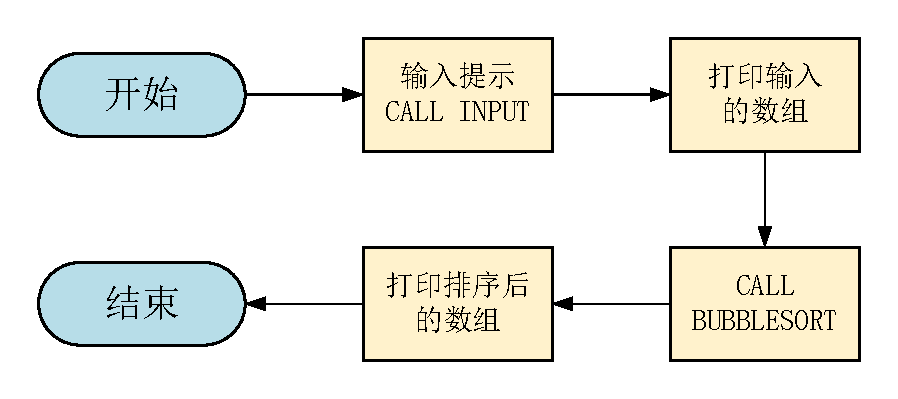
\includegraphics[width=16cm]{t1.pdf}
	\caption{题目 1 主体设计流程图}\label{pro:t1}
\end{figure}

\begin{figure}[hbtp]
	\centering
	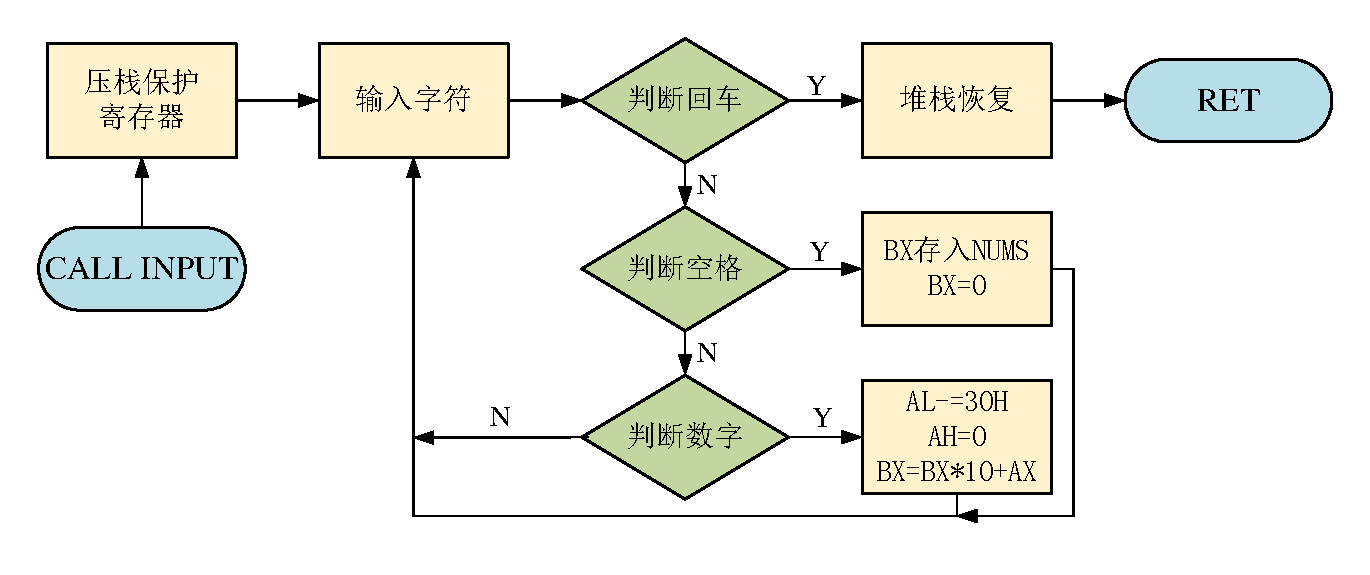
\includegraphics[width=16cm]{t1_input.pdf}
	\caption{题目 1 子程序 INPUT 设计流程图}\label{pro:t1_input}
\end{figure}

\begin{figure}[hbtp]
	\centering
	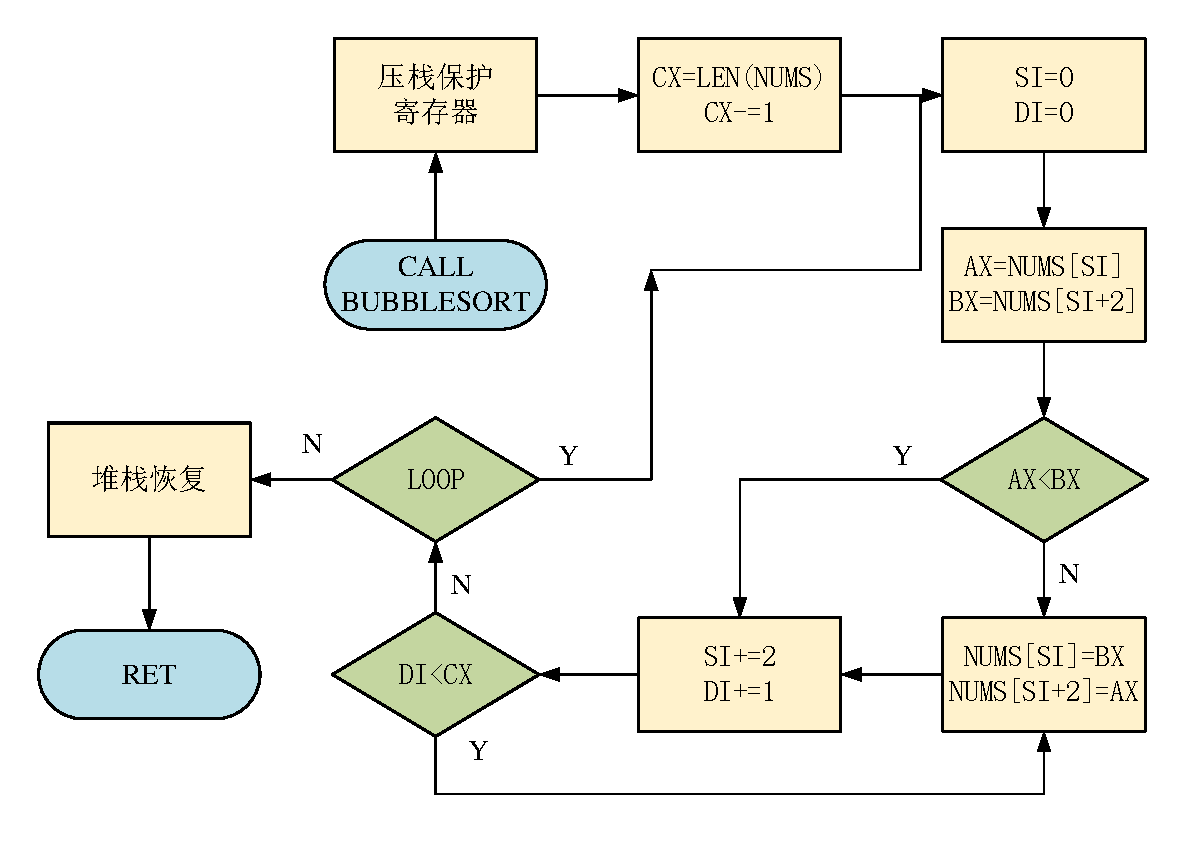
\includegraphics[width=16cm]{t1_bbsort.pdf}
	\caption{题目 1 子程序 BUBBLESORT 设计流程图}\label{pro:t1_bbsort}
\end{figure}

\subsection{题目 2 方案}

题目 2 主体设计流程图如图 \ref{pro:t2} 所示。

\begin{figure}[hbtp]
	\centering
	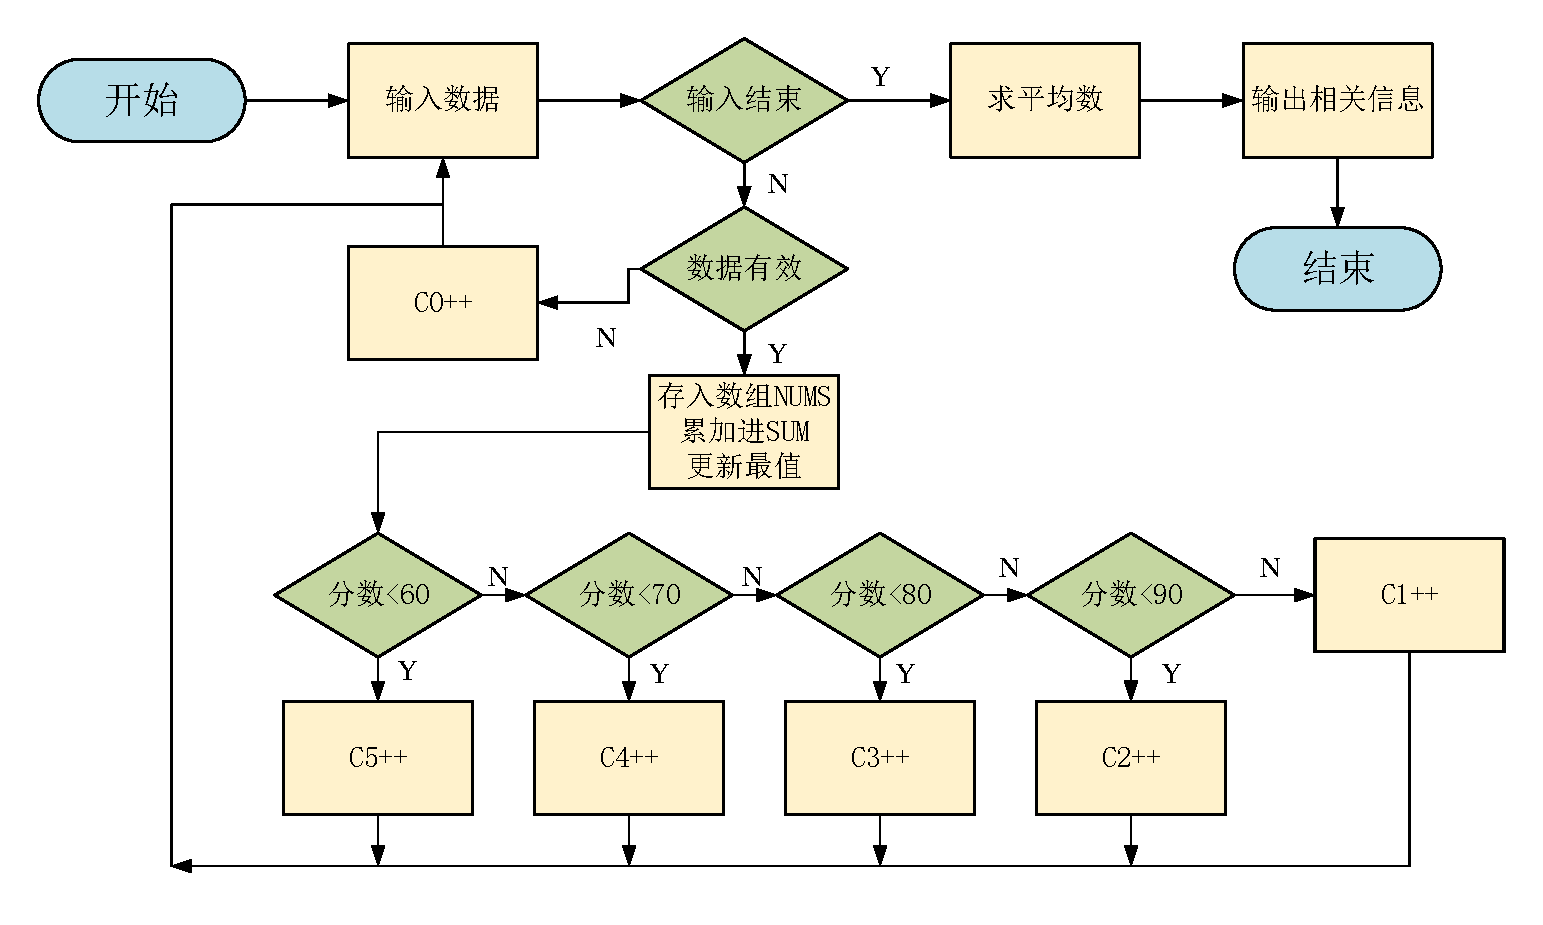
\includegraphics[width=16cm]{t2.pdf}
	\caption{题目 2 主体设计流程图}\label{pro:t2}
\end{figure}

\subsection{题目 3 方案}

题目 3 主体设计流程图如图 \ref{pro:t3} 所示,题意即在原串中查找模式串。

\begin{figure}[hbtp]
	\centering
	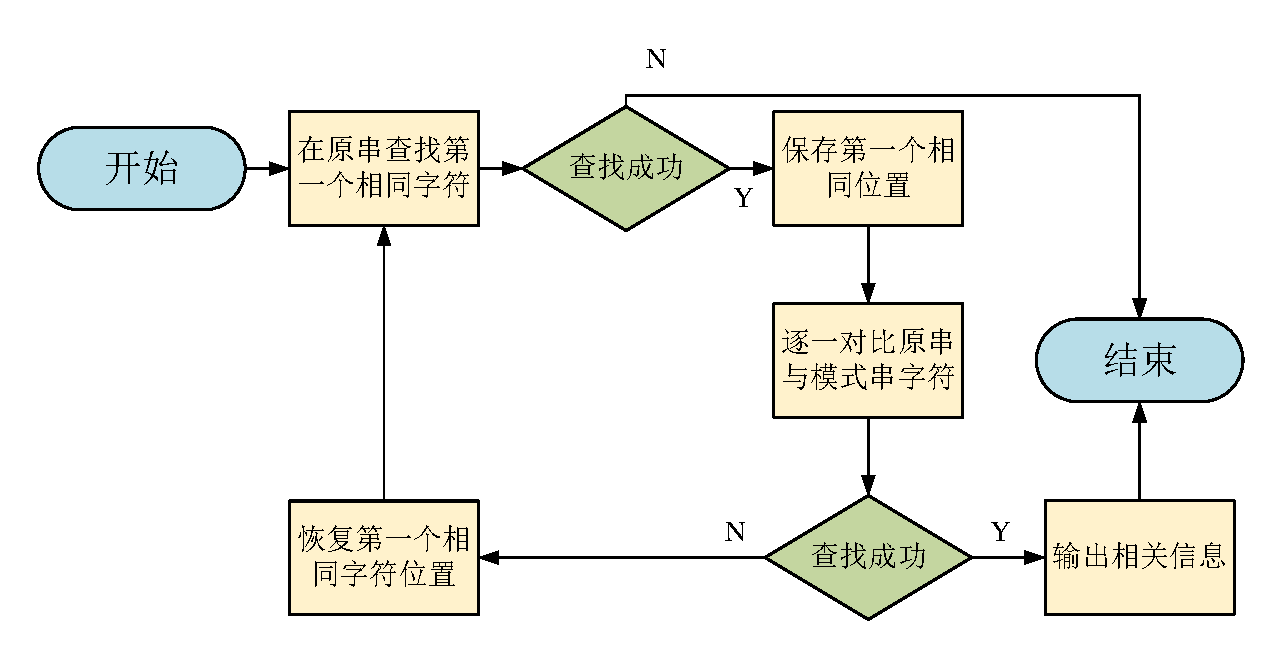
\includegraphics[width=16cm]{t3.pdf}
	\caption{题目 3 主体设计流程图}\label{pro:t3}
\end{figure}

\section{实验结果与分析}

\begin{itemize}
	\item 题目 1 输入的数据为 $65535\ 1\ 99\ 0\ 8888\ 555\ 321\ 10000\ 23\ 101$,其实验结果如图 \ref{fig:out1} 所示。
	\item 题目 2 输入的数据为 $67\ 88\ 97\ 94\ 78\ 91\ 74\ 68\ 101\ 9\ asd345\ 10000\ 57\ 73$,其中有效数字的平均数为 $\displaystyle\frac{67+88+97+94+78+91+74+68+9+57+73}{11}=72.363636\approx72.4$,其实验结果如图 \ref{fig:out2} 所示。
	\item 题目 3 无输入数据,偏移地址从 0 开始,则学号在 3 处找到,姓名在 18 处找到,其实验结果如图 \ref{fig:out3} 所示。
\end{itemize}

\begin{figure}[hbtp]
	\centering
	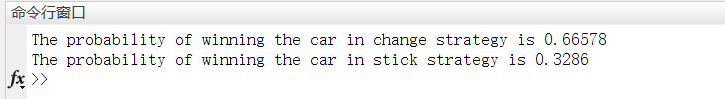
\includegraphics[width=16cm]{out1.png}
	\caption{题目 1 实验结果图}\label{fig:out1}
\end{figure}

\begin{figure}[hbtp]
	\centering
	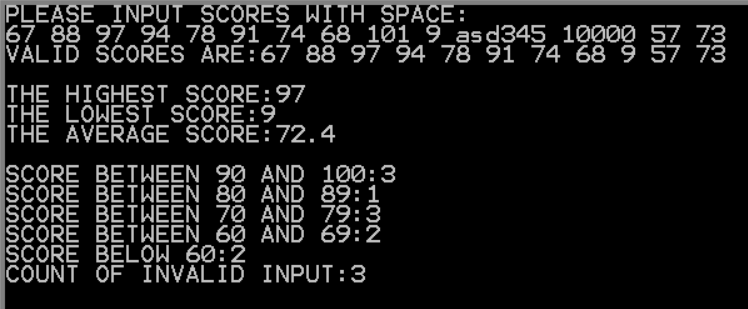
\includegraphics[width=16cm]{out2.png}
	\caption{题目 2 实验结果图}\label{fig:out2}
\end{figure}

\begin{figure}[hbtp]
	\centering
	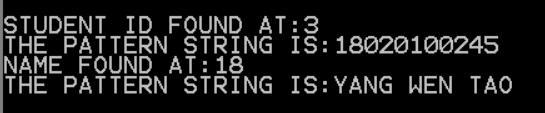
\includegraphics[width=16cm]{out3.png}
	\caption{题目 3 实验结果图}\label{fig:out3}
\end{figure}


\section{实验的收获及心得}

通过本次实验,我进一步加深了对分支程序设计、循环程序设计和子程序设计的理解,掌握了利用汇编语言实现排序的基本方法和汇编语言中的字符串相关操作,能够较好地将思路转化为流程图,进一步熟悉了 \LaTeX 排版和 Viso 绘图技巧。有一点感触最深的是,用高级语言实现起来相当容易的算法,用汇编语言实现却会复杂很多,从机器码到汇编语言,从汇编语言到高级语言,是两个非常大的跨越,每一步都大大解放了生成力,学习汇编语言可以让我们更加了解过去的编写程序的方法和加深理解现代计算机的一些概念,对未来的程序设计理解是非常有帮助的。

\section{实验代码}

\subsection{题目 1 代码}

\begin{lstlisting}[language={[x86masm]Assembler}]
DATA SEGMENT
    STR1 DB 'PLEASE INPUT NUMBERS WITH SPACE:(0-65535)',13,10,'$'   
    STR2 DB 13,10,'INPUT ERROR! PLEASE INPUT AGAIN:','$'
    STR3 DB 13,10,'INPUT NUMBERS ARE:','$'
    STR4 DB 13,10,'SORTED NUMBERS ARE:','$'
    NUMS DW 100 DUP(?)
DATA ENDS

STACK SEGMENT STACK 'STACK'
    DW 256 DUP(?)
STACK ENDS

CODE SEGMENT
    ASSUME CS:CODE,DS:DATA,SS:STACK
START:
    MOV AX, DATA
    MOV DS, AX
    MOV AX, STACK
    MOV SS, AX
    
    XOR SI, SI
    XOR DI, DI
    
    MOV DX, OFFSET STR1
    MOV AH, 9
    INT 21H
    CALL INPUT
    
    MOV CX, DI
    PUSH CX
    
    MOV DX, OFFSET STR3
    MOV AH, 9
    INT 21H
    XOR DI, DI
FOR1:
    CALL PRINT
    ADD DI, 2
    LOOP FOR1
    
    POP CX
    CALL BUBBLESORT
    
    MOV DX, OFFSET STR4
    MOV AH, 9
    INT 21H
    XOR DI, DI
FOR2:
    CALL PRINT
    ADD DI, 2
    LOOP FOR2
    
    MOV AH, 4CH
    INT 21H
    
; 输入子程序
INPUT PROC NEAR
    PUSH AX
    PUSH BX
    PUSH CX
    PUSH DX
    
    XOR BX, BX
    
CHECK: ; 输入检查
    MOV AH, 1
    INT 21H
    CMP AL, 0DH ; 回车
    JZ IN_OVER
    CMP AL, 20H ; 空格
    JZ NUMBER
    SUB AL, 30H
    JL IN_ERROR
    CMP AL, 09H
    JG IN_ERROR
    MOV AH, 0
    XCHG AX, BX
    MOV CX, 10
    MUL CX
    JC IN_ERROR
    ADD AX, BX
    JC IN_ERROR ; 大于 65535 输入错误
    XCHG AX, BX
    JMP CHECK
    
NUMBER: ; 输入为数字
    MOV NUMS[SI], BX
    ADD SI, 2
    INC DI
    XOR BX, BX
    JMP CHECK
IN_ERROR: ; 错误提示
    XOR BX, BX
    MOV DX, OFFSET STR2
    MOV AH, 9
    INT 21H
    JMP CHECK    
IN_OVER: ; 输入结束
    MOV NUMS[SI], BX
    INC DI
    XOR BX, BX
    
    POP DX
    POP CX
    POP BX
    POP AX
    RET
INPUT ENDP

; 排序子程序
BUBBLESORT PROC NEAR
    PUSH AX
    PUSH BX
    PUSH CX

    DEC CX
L1:
    XOR SI, SI
    XOR DI, DI
L2:
    MOV AX, NUMS[SI]
    MOV BX, NUMS[SI+2]
    CMP AX, BX
    JB L3
    MOV NUMS[SI], BX
    MOV NUMS[SI+2], AX
L3:
    ADD SI, 2
    INC DI
    CMP DI, CX
    JB L2
    LOOP L1
    
    POP CX
    POP BX
    POP AX
    RET       
BUBBLESORT ENDP

; 输出一个数子程序
PRINT PROC NEAR
    PUSH AX
    PUSH BX
    PUSH CX
    PUSH DX
    
    MOV AX, NUMS[DI]
    MOV BX, 10
    MOV CX, 0
INIT:
    XOR DX, DX
    DIV BX ; 商 AX 余 DX
    INC CX
    PUSH DX
    CMP AX, 0
    JNZ INIT
OUTPUT:
    POP DX
    OR DX, 30H
    MOV AH, 2
    INT 21H
    LOOP OUTPUT
    
    MOV DL, 20H
    MOV AH, 2
    INT 21H
    
    POP DX
    POP CX
    POP BX
    POP AX
    RET        
PRINT ENDP

CODE ENDS
END START
\end{lstlisting}

\subsection{题目 2 代码}

\begin{lstlisting}[language={[x86masm]Assembler}]
DATA SEGMENT
    STR1 DB 'PLEASE INPUT SCORES WITH SPACE:',13,10,'$'
    STR10 DB 13,10,'VALID SCORES ARE:','$'
    STR2 DB 13,10,13,10,'THE HIGHEST SCORE:','$'
    STR3 DB 13,10,'THE LOWEST SCORE:','$'
    STR4 DB 13,10,'THE AVERAGE SCORE:','$'
    STR5 DB 13,10,13,10,'SCORE BETWEEN 90 AND 100:','$'
    STR6 DB 13,10,'SCORE BETWEEN 80 AND 89:','$'
    STR7 DB 13,10,'SCORE BETWEEN 70 AND 79:','$'
    STR8 DB 13,10,'SCORE BETWEEN 60 AND 69:','$'
    STR9 DB 13,10,'SCORE BELOW 60:','$'
    STR0 DB 13,10,'COUNT OF INVALID INPUT:','$' 
    NUMS DW 100 DUP(?)
    MAXS DW 0 ; HIGHEST SCORE
    MINS DW 100 ; LOWEST SCORE
    SUM DW 0 ; SUM OF SCORES
    C1 DW 0 ; 90-100
    C2 DW 0 ; 80-89
    C3 DW 0 ; 70-79
    C4 DW 0 ; 60-69
    C5 DW 0 ; 0-59
    C0 DW 0 ; INVALID 
DATA ENDS

STACK SEGMENT STACK 'STACK'
    DW 256 DUP(?)    
STACK ENDS

CODE SEGMENT
    ASSUME CS:CODE,DS:DATA,SS:STACK
START:
    MOV AX, DATA
    MOV DS, AX
    MOV AX, STACK
    MOV SS, AX
    
    XOR SI, SI
    XOR DI, DI
    
    MOV DX, OFFSET STR1
    MOV AH, 9
    INT 21H
    CALL INPUT
    
    MOV CX, DI
    PUSH CX
    
    MOV DX, OFFSET STR10 ; VALID SCORES
    MOV AH, 9
    INT 21H
    XOR DI, DI
FOR1:
    LEA SI, NUMS[DI]
    CALL PRINT
    MOV DL, 20H
    MOV AH, 2
    INT 21H
    ADD DI, 2
    LOOP FOR1
    POP CX
    
    MOV DX, OFFSET STR2 ; 最高分
    MOV AH, 9
    INT 21H
    LEA SI, MAXS
    CALL PRINT
    
    MOV DX, OFFSET STR3 ; 最低分
    MOV AH, 9
    INT 21H
    LEA SI, MINS
    CALL PRINT
    
    MOV DX, OFFSET STR4 ; 平均分
    MOV AH, 9
    INT 21H
    XOR DX, DX
    MOV AX, SUM
    DIV CX
    MOV SUM, AX
    LEA SI, SUM
    CALL PRINT ; 整数部分
    
    MOV BX, 10
    MOV AX, DX
    MUL BX
    DIV CX
    MOV SUM, AX
    SHL DX, 1
    CMP DX, CX
    JL NOCARRY
    INC SUM  
NOCARRY:
    LEA SI, SUM
    
    MOV DL, 2EH
    MOV AH, 2
    INT 21H 
    CALL PRINT ; 小数部分
    
    MOV DX, OFFSET STR5 ; 90-100
    MOV AH, 9
    INT 21H
    LEA SI, C1
    CALL PRINT
    
    MOV DX, OFFSET STR6 ; 80-89
    MOV AH, 9
    INT 21H
    LEA SI, C2
    CALL PRINT
    
    MOV DX, OFFSET STR7 ; 70-79
    MOV AH, 9
    INT 21H
    LEA SI, C3
    CALL PRINT
    
    MOV DX, OFFSET STR8 ; 60-69
    MOV AH, 9
    INT 21H
    LEA SI, C4
    CALL PRINT
    
    MOV DX, OFFSET STR9 ; 0-59
    MOV AH, 9
    INT 21H
    LEA SI, C5
    CALL PRINT
    
    MOV DX, OFFSET STR0 ; INVALID
    MOV AH, 9
    INT 21H
    LEA SI, C0
    CALL PRINT
    
    MOV AH, 4CH
    INT 21H
    
; 输入子程序
INPUT PROC NEAR
    PUSH AX
    PUSH BX
    PUSH CX
    PUSH DX
    
    XOR BX, BX
    XOR DX, DX
    
CHECK:
    MOV AH, 1
    INT 21H
    CMP AL, 0DH ; 回车    
    JZ IN_OVER
    CMP AL, 20H ; 空格
    JZ CONTENT
    CMP DL, 0
    JNZ CHECK ; 已经不合法不继续比较
    SUB AL, 30H
    JL IN_ERROR
    CMP AL, 09H
    JG IN_ERROR
    MOV AH, 0
    XCHG AX, BX
    MOV CX, 10
    MUL CX
    ADD AX, BX
    CMP AX, 100
    JG IN_ERROR
    XCHG AX, BX
    JMP CHECK
CONTENT:
    CMP DL, 0
    JNZ CASE0
    MOV NUMS[SI], BX
    ADD SI, 2
    INC DI
    ADD SUM, BX
    CMP MAXS, BX
    JL UPDATE_MAX
    CMP MINS, BX
    JG UPDATE_MIN 
COMPARE:
    CMP BX, 60
    JL CASE5
    CMP BX, 70
    JL CASE4
    CMP BX, 80
    JL CASE3
    CMP BX, 90
    JL CASE2
    JMP CASE1
UPDATE_MAX: ; UPDATE HIGHEST SCORE
    MOV MAXS, BX
    CMP MINS, BX
    JG UPDATE_MIN
    JMP COMPARE
UPDATE_MIN: ; UPDATE LOWEST SCORE
    MOV MINS, BX
    JMP COMPARE
CASE0: ; INVALID
    INC C0
    JMP OVER
CASE1: ; 90-100
    INC C1
    JMP OVER
CASE2: ; 80-89
    INC C2
    JMP OVER
CASE3: ; 70-79
    INC C3
    JMP OVER
CASE4: ; 60-69
    INC C4
    JMP OVER
CASE5: ; 0-59
    INC C5
    JMP OVER    
CONTINUE:
    XOR BX, BX
    XOR DL, DL
    JMP CHECK
IN_ERROR:
    XOR BX, BX
    INC DL ; DL != 0 存在无效数字
    JMP CHECK
IN_OVER:
    INC DH
    CMP DL, 0
    JNZ OVER
    MOV NUMS[SI], BX
    INC DI
    
    ; 最后一个数相关操作
    ADD SUM, BX
    CMP MAXS, BX
    JL UPDATE_MAX
    CMP MINS, BX
    JG UPDATE_MIN
    JMP COMPARE
OVER:
    CMP DH, 0
    JZ CONTINUE
        
    POP DX
    POP CX
    POP BX
    POP AX
    RET
INPUT ENDP

PRINT PROC NEAR
    PUSH AX
    PUSH BX
    PUSH CX
    PUSH DX
    
    MOV AX, [SI]
    MOV BX, 10
    MOV CX, 0
INIT:
    XOR DX, DX
    DIV BX ; 商 AX 余 DX
    INC CX
    PUSH DX
    CMP AX, 0
    JNZ INIT
OUTPUT:
    POP DX
    OR DX, 30H
    MOV AH, 2
    INT 21H
    LOOP OUTPUT
    
    POP DX
    POP CX
    POP BX
    POP AX
    RET
PRINT ENDP

CODE ENDS
END START
\end{lstlisting}

\subsection{题目 3 代码}

\begin{lstlisting}[language={[x86masm]Assembler}]
DATA SEGMENT
    STRING DB '***','18020100245','YANG','YANG WEN TAO','***','$'    
    SID DB '18020100245','$'
    SNAME DB 'YANG WEN TAO','$'
    STR1 DB 13,10,'STUDENT ID FOUND AT:','$'
    STR2 DB 13,10,'NAME FOUND AT:','$'
    STR DB 13,10,'THE PATTERN STRING IS:','$'
    LEN DW 33 ; 原串长度
    LEN1 DW 11 ; 学号长度
    LEN2 DW 12 ; 姓名长度
    ADDR DW 1
DATA ENDS

STACK SEGMENT STACK 'STACK'
    DW 64 DUP(?)    
STACK ENDS

CODE SEGMENT
    ASSUME CS:CODE,DS:DATA,ES:DATA,SS:STACK
START:
    MOV AX, DATA
    MOV DS, AX
    MOV ES, AX
    MOV AX, STACK
    MOV SS, AX
    
    
    MOV DX, OFFSET STR1 ; SID
    MOV AH, 9
    INT 21H
    ; 求串长度
    ; LEA SI, STRING
    ; CALL STRLEN
    ; MOV LEN, DI
    
    LEA SI, SID
    MOV DX, LEN1 ; DX 存储模式串长度
    
    CALL SEARCH
    LEA SI, ADDR
    CALL PRINT
    
    MOV DX, OFFSET STR ; 打印模式串
    MOV AH, 9
    INT 21H
    
    LEA SI, STRING
    ADD SI, ADDR
    MOV CX, LEN1
    CALL STRPRT
                          
    MOV DX, OFFSET STR2 ; SNAME
    MOV AH, 9
    INT 21H
    
    LEA SI, SNAME
    MOV DX, LEN2
    
    CALL SEARCH
    LEA SI, ADDR
    CALL PRINT
    
    MOV DX, OFFSET STR ; 打印模式串
    MOV AH, 9
    INT 21H
    
    LEA SI, STRING
    ADD SI, ADDR
    MOV CX, LEN2
    CALL STRPRT
    
    MOV AH, 4CH
    INT 21H
    
SEARCH PROC NEAR: 
    PUSH AX
    PUSH CX
    PUSH DX
    
    LEA DI, STRING
    MOV CX, LEN
    DEC DX
    MOV AL, [SI]
    
    CLD
COMPARE:    
    REPNZ SCASB ; 找到第一个相同字符
    JNZ NOTFOUND
    PUSH SI
    INC SI
    PUSH CX
    PUSH DI ; 保存第一个相同的位置+1
    MOV CX, DX
    REPZ CMPSB
    POP DI
    POP CX
    POP SI
    JNZ COMPARE
FOUND:
    SUB DI, 1
    MOV ADDR, DI    
NOTFOUND:

    POP DX
    POP CX
    POP AX
    RET
SEARCH ENDP

STRLEN PROC NEAR
    PUSH AX
    PUSH CX
    
    XOR CX, CX
COUNT:
    MOV AL, [SI]
    CMP AL, '$'
    JZ CNTEND
    INC CX
    INC SI
    JMP COUNT
CNTEND:
    MOV DI, CX
    
    POP CX
    POP AX
    RET    
STRLEN ENDP

STRPRT PROC NEAR ; 在原串中显示模式串
    PUSH AX
    PUSH CX
    
PRT:
    MOV DL, [SI]
    MOV AH, 2    
    INT 21H
    INC SI
    LOOP PRT
    
    POP CX
    POP AX
    RET    
STRPRT ENDP

PRINT PROC NEAR
    PUSH AX
    PUSH BX
    PUSH CX
    PUSH DX
    
    MOV AX, [SI]
    MOV BX, 10
    MOV CX, 0
INIT:
    XOR DX, DX
    DIV BX ; 商 AX 余 DX
    INC CX
    PUSH DX
    CMP AX, 0
    JNZ INIT
OUTPUT:
    POP DX
    OR DX, 30H
    MOV AH, 2
    INT 21H
    LOOP OUTPUT
    
    POP DX
    POP CX
    POP BX
    POP AX
    RET
PRINT ENDP

CODE ENDS
END START
\end{lstlisting}

% % 参考文献,此处以 MLA 引用格式为例

%\begin{thebibliography}{9}
%\end{thebibliography}

% % \includepdf[pages={1,2}]{Memo.pdf} 
% 可以直接导入pdf页面
%\newpage
%\begin{appendices}  % 附录环境
%\section{核心层}\label{subsec:B}
%\end{appendices}
\end{document}  % 结束